\documentclass[12pt]{article}
\usepackage[utf8]{inputenc} %mogu sa ovim pisati ščđžć
\usepackage{extsizes} %mogu koristi visinu fonta koju želim 	%

%\usepackage{hyperref} 					
\usepackage{hhline}
\usepackage{tikz}
\usepackage{amsmath}
\usepackage{listings}
%\usepackage{xcolor}
\lstset { %
	language=C++,breaklines=true,showstringspaces=false,
	backgroundcolor=\color{black!5}, % set backgroundcolor
	keywordstyle=\color{red},
	commentstyle=\color{blue},
	basicstyle=\sffamily,% basic font setting
	numbers=left,%
	numberstyle={\tiny \color{black}},% size of the numbers
	numbersep=9pt, % this defines how far the numbers are from the text
}

\usepackage{times}

\usepackage{geometry} %štimanje margina
\geometry{textwidth=18cm}
\geometry{textheight=22cm}

\usepackage[english]{babel}

\usepackage{array} %za tabele
\newcolumntype{P}[1]{>{\centering\arraybackslash}p{#1}}

\usepackage{enumitem}

\usepackage{caption}
\usepackage{subcaption}

\usepackage{multicol} % multikolone
\usepackage{graphicx}
\usepackage{setspace}

\usepackage[obeyspaces]{url} % for adding paths to a folder
\graphicspath{{./figures/}}

%\path{{./Data/}} % adddig a path to a folder

\usepackage{wrapfig} %wraps figure
\usepackage{lipsum}  %fills text around figure

\usepackage{bm}  %mogu pisati boldirane formule sa simbolima

\usepackage{amssymb} % za pisannje skupova

\usepackage[usestackEOL]{stackengine} %za piasanje front page-a
\numberwithin{equation}{section}

%\makeatletter
%\renewcommand{\@seccntformat}[1]{}
%\makeatother  % removes numbers from sections but keeps the references
\usepackage{fancyhdr}
\pagestyle{fancy}
\fancyhf{}
\rhead{\scriptsize \hspace*{0cm}  Thesis topic: Graph-Based Keyword Extraction from
 \\ Scientific Paper Abstracts using Word Embeddings}
\lhead{\scriptsize Universit\`a  di Bologna \\ Department of Computer Science and Engineering}
\fancyheadoffset{1cm} % to offset the header by some distance 


\usepackage{epsfig}
\usepackage{multirow}
\usepackage{pdfpages}
\setcounter{MaxMatrixCols}{20} % maksimalan broj kolona na 20
\usepackage{float} % da slike nisu poremećene
\usepackage[figurename=Figure]{caption} % mijenja ime sa figure u slika
\usepackage[tablename=Table]{caption} % mijenja ime sa figure u slika

\usepackage{chngcntr}
%\counterwithout{figure}{chapter} % stavlja bojeve unutar captiona slike

\usepackage{colortbl} % color in tables

\addto\captionsenglish{% Replace "english" with the language you use
	\renewcommand{\contentsname}% Promjena naziva content
	{Content}%
}

\usepackage{etoolbox}
%\patchcmd{\thebibliography}{\section*{\refname}}{}{}{} % smakinje ime references

%\usepackage[colorlinks=true, linkcolor = cyan]{hyperref}
\usepackage{hyperref}

%rotating picture
\usepackage{lscape}
\usepackage{rotating}

% tilda
\usepackage{undertilde}

%%coloring links
%\usepackage{hyperref}
%\hypersetup{
	%	colorlinks = true,
	%	linkbordercolor = [white],
	%	linkcolor = [magenta]
	%}

%\usepackage[colorlinks]{hyperref}
%\hypersetup{colorlinks=true, linkcolor=cyan,linkbordercolor=red}

%matlab
\usepackage{listings}
\usepackage{color} %red, green, blue, yellow, cyan, magenta, black, white
\definecolor{mygreen}{RGB}{28,172,0} % color values Red, Green, Blue
\definecolor{mylilas}{RGB}{170,55,241}


\lstset{
	language=Matlab,
	basicstyle=\footnotesize\ttfamily,
	breaklines=true,%
	morekeywords={matlab2tikz},
	keywordstyle=\color{blue},%
	morekeywords=[2]{1}, keywordstyle=[2]{\color{black}},
	identifierstyle=\color{black},%
	stringstyle=\color{mylilas},
	commentstyle=\color{mygreen},%
	showstringspaces=false,%without this there will be a symbol in the places where there is a space
	numbers=left,%
	numberstyle={\tiny \color{black}},% size of the numbers
	numbersep=9pt, % this defines how far the numbers are from the text
	emph=[1]{for,end,break},emphstyle=[1]\color{red}, %some words to emphasise
	emph=[2]{word1,word2}, emphstyle=[2]{style},   
}

\addto\captionsenglish{% Replace "english" with the language you use
	\renewcommand{\contentsname}% Promjena naziva content
	{Contents}%
}

% stil numerisanja stranica
\usepackage{lastpage}
\cfoot{Page \thepage \hspace{1pt} of \pageref{LastPage}}

\usepackage{etoolbox}
\patchcmd{\thebibliography}{\section*{\refname}}{}{}{} % smakne ime references

% za pisanje pseudokoda
\usepackage[plain]{algorithm2e}
%\usepackage{algorithmic}
%\usepackage{algpseudocode}
%\usepackage{algorithmicx}
%\usepackage{algorithm}
%\usepackage{algpseudocode}
%\algnewcommand\algorithmicinput{\textbf{Function:}}
%\algnewcommand\Function{\item[\algorithmicinput]}
%\usepackage{capt-of}
\SetAlgorithmName{Pseudocode}

%\renewcommand{\@algocf@capt@plain}{top}% formerly {bottom}

\makeatletter
\newenvironment{breakablealgorithm}
{% \begin{breakablealgorithm}
		\begin{center}
			\refstepcounter{algorithm}% New algorithm
			\hrule height.8pt depth0pt \kern2pt% \@fs@pre for \@fs@ruled
			\renewcommand{\caption}[2][\relax]{% Make a new \caption
				{\raggedright\textbf{\fname@algorithm~\thealgorithm} ##2\par}%
				\ifx\relax##1\relax % #1 is \relax
				\addcontentsline{loa}{algorithm}{\protect\numberline{\thealgorithm}##2}%
				\else % #1 is not \relax
				\addcontentsline{loa}{algorithm}{\protect\numberline{\thealgorithm}##1}%
				\fi
				\kern2pt\hrule\kern2pt
			}
		}{% \end{breakablealgorithm}
		\kern2pt\hrule\relax% \@fs@post for \@fs@ruled
	\end{center}
}
\makeatother

\makeatletter
\newenvironment{breakalgo}[2][alg:\thealgorithm]{%
	\def\@fs@cfont{\bfseries}%
	\let\@fs@capt\relax%
	\par\noindent%
	\medskip%
	\rule{\linewidth}{.8pt}%
	\vspace{-3pt}%
	\captionof{algorithm}{#2}\label{#1}%
	\vspace{-1.7\baselineskip}%
	\noindent\rule{\linewidth}{.4pt}%
	\vspace{-1.3\baselineskip}%
}{%
	\vspace{-.75\baselineskip}%
	\rule{\linewidth}{.4pt}%
	\medskip%
}
\makeatother


\captionsetup{font=small}
\newcommand*{\matlab}{\textsc{Matlab}}
\newcommand*{\altmatlab}{{\mdseries\matlab}} 

\usepackage{xcolor}

\newsavebox{\bmatrixbox}
\newenvironment{colorbmatrix}
{\begin{lrbox}{\bmatrixbox}
		\mathsurround=0pt
		$\displaystyle
		\begin{bmatrix}}
		{\end{bmatrix}$%
	\end{lrbox}%
	\usebox{\bmatrixbox}%
	\kern-\wd\bmatrixbox
	\makebox[0pt][l]{$\left[\vphantom{\usebox{\bmatrixbox}}\right.$}%
	\kern\wd\bmatrixbox
}

\usepackage [autostyle, english = american]{csquotes}
\MakeOuterQuote{"}


\begin{document}
	
	\begin{titlepage}
		\begin{center}
			
			{\Large ALMA MATER STUDIORUM \\ UNIVERSIT\`A  DI BOLOGNA \\}
			\vspace{0.4cm} 
			\hrule
			\vspace{0.4cm} 
			{\Large DEPARTMENT OF COMPUTER SCIENCE AND ENGINEERING \\} 
			{\Large ARTIFICIAL INTELLIGENCE \\}
			\vspace{0.4cm} 
			\hrule
			\vspace{1cm}
			{\Large MASTER THESIS}\\[0.4cm]
			{\large in} \\[0.4cm]
			{\Large Natural Language Processing}\\[1cm]
			
			\hrule
			\vspace{0.4cm}
			
			{\Huge Graph-Based Keyword Extraction from}\\[0.3cm]
			{\Huge Scientific Paper Abstracts using Word Embeddings}
			\vspace{0.4cm}
			
			\hrule
			\vspace{2cm}
			
			{\large Author:}\\
			{\large Dinno Koluh\\}
			
			\vspace{2cm}
			
			{\large Supervisor:}\\[0.1cm]
			{\large Prof. Paolo Torroni}\\[0.4cm]
			
			{\large Co-Supervisor:}\\[0.1cm]
			{\large Dr. Federico Ruggeri}
			
			\vspace{2cm} 
			{\large Bologna,}\\[0.1cm] 
			{\large December 2023.}
			
		\end{center}
	\end{titlepage}
	\newpage
	\newgeometry{textwidth=16cm, textheight=22cm}
	\thispagestyle{empty}
	
	\begin{spacing}{1.5}
	\section*{Abstract}
	In the era of information overload it became essential to efficiently extract concise, precise and quality information from large texts. One aspect of information extraction is keyword extraction where large texts are represented as sets of tokens i.e. keywords. This prospect of keyword extraction is paramount to researchers as they deal with huge numbers of scientific papers, and having a good and concise representation of those papers is essential for them. This thesis paper addresses that problem in the realm of natural language processing (NLP). \\
	Using core concepts of NLP and modeling texts as graphs, we are going to build a model for the automatic extraction of keywords. This is done in an unsupervised manner as the importance of a word is calculated through the position and weights associated with respective words in the graph. The first metric used to calculate the graph weights are co-occurrence matrices and the other metric are word embeddings. Word embeddings became a crucial way of representing the semantic information of words as dense vectors. \\
	The results of this paper were compared with keywords that were provided by authors of scientific papers in the area of computer science which act as the ground truth, but crucially are not a component in the model construction, but just serve as a verifier of the model's accuracy.
	
	\textbf{Keywords}: NLP, keyword extraction, scientific papers, graphs, word-embeddings
	
	\newpage
	\pagestyle{empty}
	\tableofcontents
	\setcounter{page}{0}
	\newpage
	%\renewcommand{\listfigurename}{Figures}
	\listoffigures
	\setcounter{page}{0}
	\pagebreak
	
	%\renewcommand{\listtablename}{Popis tabela}
%	\listoftables
%	\thispagestyle{empty}
%	\setcounter{page}{0}
%	\pagebreak
	
	\newpage
	\pagestyle{fancy}
	%\thispagestyle{empty}
	\section{Introduction and Motivation}
	Natural Language Processing (NLP) is a subfield or Artificial Intelligence (AI) and linguistics that has a focus on the interaction between computers and human languages. This is mostly restricted to written language as other fields (like Speech Processing) deal with spoken language (using audio instead of textual features). In the past decade NLP has seen huge attention with the introduction of some key concepts like \textit{word-embeddings} \cite{word-embedding-survey} (which we are going to use) and \textit{transformers} \cite{transformers-survey}. At the moment of writing of this paper, NLP is the subfield of AI that has the most resources invested into it, mostly in research and development, with new large language models (LLMs) coming out on a daily basis. Our focus will be a bit shifted from Deep Neural Network (DNN) models and more to traditional Machine Learning (ML) models. \\
	NLP has many subfields and application areas such as:
	\begin{itemize}
		\item Text classification
		\item Information retrieval
		\item Automatic translation
		\item Speech analysis 
		\item Question answering
		\item Conversational agents
		\item Sentiment analysis
	\end{itemize} 
	The field we are going to be working on will be \textbf{information retrieval}, more precisely \textit{keyword extraction}. Keyword (keyphrase) extraction is the automatic selection of important and topical phrases from the body of a document \cite{keyword-extraction-0}. Scientific papers are usually the area where keywords are frequently used as researchers use them for a quick overview of papers and also sorting papers into different categories. This is the topic we are going to be working on as well. The keywords are going to be extracted from the abstracts of the scientific papers. One detail we should address that will be important later is the distinction between \textit{keywords} and \textit{keyphrases}. Keywords would be single words or at most MWEs (Multi-Word expressions, i.e. "deep learning") while keyphrases are more complicated entities comprised of several words and they act as a single unit (e.g. the phrase "scientific paper" would be a keyphrase). When doing keyword extraction we might have as an output a combination of both, keywords and keyphrases. Usually keyphrases carry more information than keywords but a combination of both as an output is most representative. From now on, when referring to \textit{keywords} it will also include \textit{keyphrases}, if not explicitly stated otherwise. \\
	The model to be used for keyword extraction is \textbf{graph-based}. The motivation behind using graphs is that graphs are a well-studied and understood concept and many practical problems can be represented with graphs. There are also a plethora of algorithms which are going to be useful for the case of instance ranking. \\
	The idea is to model words in a paper abstract as nodes of a graph. Not all the words in the abstract should be included, as keywords are usually composed of a combination of nouns and adjectives (e.g. scientific[ADJ] paper[N]). This means that some preprocessing of the raw text will be required, especially when dealing with MWEs. We will speak about this in the next chapter. \\
	As stated, the nodes of the graph will be modeled as words, but the question comes on how to model the edges of the graph? \\
	It starts from the assumption that words that occur in the same context tend to carry a similar meaning. The idea is to use a \textbf{sliding window} of some predefined size and words that are in that window are connected with and edge. In that way the final graph carries semantic (the meaning of words) information of the input text. The number of occurrences when sliding the window over the entire text will give us the initial graph weights. To solidify this relationship another metric that we will use are word embeddings. Word embeddings are essentially a way of representing words as vectors of numbers. We will dive more deeply into how word embeddings are computed ans used but for now we can assume that word embeddings are vectors of numbers and that these vectors carry semantic information of the corresponding word. This means that words that have a similar meaning (whatever that might mean in some general picture) also have similar vector representations and that we can use the usual mathematical tools on these vectors like the dot product which means that we can actually measure the similarity between words. \\
	We now have the complete representation of the input text as a graph. Now we need to somehow rank the nodes according to the graph edges and weights. We can refer to the ranking procedure as to finding the importance of each node. There are several algorithms which can find the importance of nodes, and we will speak in more detail about them later, but for now can assume we have a black box which takes in the graph representation of the abstract as described before and gives us all the nodes (word) ranked by their importance. \\
	We now have a list of the most important words, but there is one more step that we can do to get a more robust output. The given output would be a list of words, but we might want to have phrases instead of keywords (e.g. the phrase "scientific paper" is more representative instead of just "paper"). We can use the words we got out from the graph and traverse the initial text for phrases in which they appear. Then based on those phrases in the initial text and the importance of the words which they are made of, we can get alongside the ranked words also the phrases in which they appear. In this way we can also generalize the problem by letting a phrase be only made up of one keyword. If it is made up of more than one keyword we can average it out, and in the end get the ranking of the specific phrases which appear in the input text. \\
	This was a rough explanation of the procedures which should give us an overview of the steps involved in developing a pipeline for the extraction of keywords from paper abstracts. In the next few chapters we are going to look in more detail in the inner workings of the steps involved. We will start with the NLP preprocessing pipeline.
	
	
	\newpage
	\section{NLP Pipeline}
	In this chapter we are going to explain the preprocessing steps needed to transform the raw input text into something that can be modeled with a graph. These preprocessing steps are going to be carried out with concepts from NLP like tokenization, sentence splitting, lemmatization, etc. All these NLP concepts used for preprocessing can be stacked into a pipeline hence the name of the chapter, \textbf{NLP pipeline}.\\
	We will explain these concepts giving examples and at the end show the whole pipeline as a schema. In the end we will have single instances of processed words which are going to be the graph nodes. Let us start!
	
	\subsection{Tokenization}
	Tokenization is the basic and most important NLP concept. Let us firstly define what a token is. A \textbf{token} is a sequence of characters grouped together as a semantic unit used for text processing \cite{stanford_NLP}. Depending on the use case,  tokens can be equivalent to words, but they don't have to. They can even be single characters but that depends on the tokenizer model used. An example of words and tokens not being equivalent is:
	\begin{center}
		I'd $\rightarrow$ [I, 'd]
	\end{center}
	In this case the word "I'd" was broken into two tokens. Depending on the specific tokenization method used, words can be broken into lower units (subwords):
	\begin{center}
		unlucky $\rightarrow$ [un, lucky]
	\end{center}
	Here, we have that the adjective "unlucky" was broken into its prefix "un" and the adjective "lucky". In this example tokenization provided a way to work with text on a granular level, breaking down words into units which might not even be real words, but in this way we are making text processing tasks more cohesive for machines. \\
	The process of \textbf{tokenization} would be the process of breaking down an input text into single tokens. As the input text inherently has whitespaces and newlines, those are usually excluded from the obtained tokens. We can look at an example sentence broken down into tokens: 
	\begin{center}
		She didn't have time. $\rightarrow$ [She, did, n't, have, time, .]
	\end{center}
	When dealing with whitespaces, tokenization is a trivial process, but when dealing with punctuations, tokenization becomes a hard problem. The reason is that sometimes punctuations should be kept, but sometimes they should be separated. In the example above, the token "time." was separated into "time" and ".", but let's take a look at this example:
	\begin{center}
		She didn't have time for Mr. Nobody. $\rightarrow$ [She, did, n't, have, time, for, Mr., Nobody, .]
	\end{center}
	In this example the period for the token "Mr." was not separated while for "Nobody." it was. This is the reason why tokenization can be ambiguous and hard to compute correctly. And there are tens of other example of ambiguities apart from punctuation marks. One solution to the problem we've seen is to keep a \textbf{lexicon} of possible ambiguous tokens so we know how to separate them.
	
	\subsection{Sentence splitting}
	Sentence splitting is the process of splitting up text into sentences. This steps is going to be important when computing co-occurrence matrices with the sliding window. The reason is that when using the sliding window we don't want to capture the end of one sentence and the beginning of the next one in the same context as they might not carry the same meaning as sentences are naturally boundaries that also we, humans, respect and take into account when reading and processing text. \\
	Sentence splitting has inherently similar problems as tokenization does as punctuation signs can be ambiguous depending on the position and the tokens surrounding the punctuation sign. Apart from punctuation signs, sentences in quotation marks inside sentence cause problems as such sentences are basically nested sentences. But for our purposes we don't expect to have many such examples in scientific paper abstracts.
	
	\subsection{MWE}
	MWE or Multi-Word Expressions are sequences of words that when grouped together carry one meaning, but when standing alone carry another. An example of an MWE is "deep learning". We see that the word "deep" and "learning" on their own carry other meanings in contrast when putting them together into a single phrase. For the purposes of this paper we need to keep these expressions together and not split them. The reason is that we are extracting keywords and keyphrases, and the keyphrase to be extracted from a paper that is written on the topic of "deep learning" is "deep learning", not "deep" and "learning". \\
	When dealing with scientific papers, we expect that they are going to have many MWEs and possibly new, non-existent MWEs. This makes the tokenization problem ever more harder because these tokens should be kept together. One solution is to again keep an MWE lexicon. Another solution, which was observed while inspecting the dataset is that novel MWEs are usually written with upper-case letters and they have an abbreviation after the MWE in parenthesis (e.g. "Introduction to Large Language Models (LLMs)") and this fact can be leveraged when dealing with MWE that are not present in the MWE lexicon. \\
	Let us see an example for MWE tokenization:
	\begin{center}
		We are discussing Machine Learning (ML) models in San Francisco. $\rightarrow$ \\
		
		[We, are, discussing, Machine Learning, (, ML, ), models, in, San Francisco, .]
	\end{center} 
	
	\subsection{Token removal based on PoS tags}
	This step is specific for our task, but PoS (Part of Speech) is a regular NLP concept. \textbf{Part of Speech} tagging is the process of giving a grammatical category tag to words based on their syntactic and semantic meaning. Basically this step assigns syntactic tags to words i.e. telling if a word is a noun, verb, adjective, etc. The question is why do we need this step?\\
	The reason is the nature of the task we are doing. Namely, keywords are usually a phrase of an adjective and verb or at most a single noun. Taking this into consideration we can substantially reduce the graph size if we just keep nouns and adjective as the possible graph nodes. There are several ways on getting PoS tags of words, like rule-based methods, statistical methods, hybrid methods, deep learning methods, etc. 
	We are not going into the inner workings of these methods, but we will just use an existing model for getting PoS tags. One of the problems when computing PoS tags is they highly depend on the context in which they occur as we can have words which are \textit{homographs} (they are spelled the same but have a different meaning) but carry different PoS tags. For example the word "developed" can be a verb and an adjective at the same time as show below:
	\begin{center}
		Japan[Noun] developed[Verb] into[Prep.] a[Det.] developed[Adj.] nation[Noun].
	\end{center}
	This is the reason why context is very important when assigning PoS tags. Deep learning and statistical methods are usually good at these context specific examples but they require quite large training datasets. \\
	An example of this step can be seen below:
	\begin{center}
		Japan developed into a developed nation. $\rightarrow$ [Japan, developed, nation, .]
	\end{center}	  
	
	\subsection{Stopword removal}
	Stopwords are common words occurring in a language that are usually filtered out during NLP tasks as they do not carry much value for the specific task. For our purposes stopword removal is essential as we are going to have many of them, and in the final ranking they will not be present in the keyphrases. The usual method of stopword removal is to build a stopword lexicon and just remove those words from the input text. An example of stopwords are: "the", "and", "in", etc. Let us see an example for stopword removal on a sentence:
	\begin{center}
		The quick brown fox jumped over the lazy dog. $\rightarrow$ [quick, brown, fox, jumped, lazy, dog, .]
	\end{center} 
	This step will come after the token removal based on PoS tags, as stopwords could carry context specific information for PoS tagging. Even though PoS tagging should take care of stopwords, we will still include this step in case some stopword slip thorough the previous step, as stopword removal is a cheap operation.
	
	\subsection{Lemmatization}
	Lemmatization is an NLP technique used to reduce words to their base form, also known as their \textit{root} or \textit{lemma}. This means that words that might be morphologically different have the same root and we want to transfer those words to their root form. Some examples of lemmatization is show below:
	\begin{center}
		am, are, is $\rightarrow$ be \\
		horses, horse, horses', horse's $\rightarrow$ horse \\
		develops, developed, developing $\rightarrow$ develop
	\end{center}
	For lemmatization to be accurate, it usually uses PoS as context is important to determine the grammatical role of a word in a sentence. This step is important as the lemma of a word may vary depending on its PoS. Lemmatization will usually transform verbs, adjectives and adverbs to their base form, but if a noun is present among a set of words (e.g. "developer" in the last example) it will keep the noun how it is as nouns are usually lemmas themselves (but it will of course strip possessive or plural forms). With the use of PoS tags and grammatical rules and dictionaries, words are mapped to their lemmas. \\
	One similar concept to lemmatization is stemming, where in the stemming process words are stripped from their suffixes and prefixes using a predefined set of rules. The problem with stemming is that it might produce non-existent words (e.g. "replacement" $\rightarrow$ "replac") which is not practical for our purposes. \\
	The reason we need lemmatization is that words that might have different forms have to be treated as the same word as in the other case we would have two different nodes in the graph that actually represent the same word. Let us see an example of this:
	\begin{center}
		Graph models were used for modeling words. $\rightarrow$ Graph model be use for model word.	
	\end{center}
	
	\subsection{Normalization}
	Normalization is the process of putting words with different forms into a single normalized form. A good example of this step is the lowercasing of all words in a sentence, otherwise we will have words which are the same but they are essentially represented as two different words. We could also look at lemmatization and stemming as parts of normalization as they also map words with different forms into a single one, but we will keep them as two separate steps. \\
	One essential normalization step will be normalizing MWE expressions into single forms. We can look at the example below:
	\begin{center}
		U.S.A., US, United States, United States of America, USA $\rightarrow$ USA
	\end{center}
	All of the words on the left essentially mean the same thing, so we can represent it by one word. We will encounter a great deal of MWE expressions in scientific papers that use acronyms and their long forms, so it is necessary to represent them as a single word. \\ 
	In the normalization process we will also include the removal of punctuation signs and other non-alphanumeric sign (e.g. \#, (, ), ?), and the expansion of clitics into their expanded form (e.g. I'd $\rightarrow$ I would).
	
	\subsection{The pipeline}
	Let us now combine all the steps of the NLP preprocessing pipeline into a single schema in Figure \ref{NLP_pipeline_label} for better readability.
	\begin{figure}[H]
		\centering
		\hspace*{-1.0cm}
		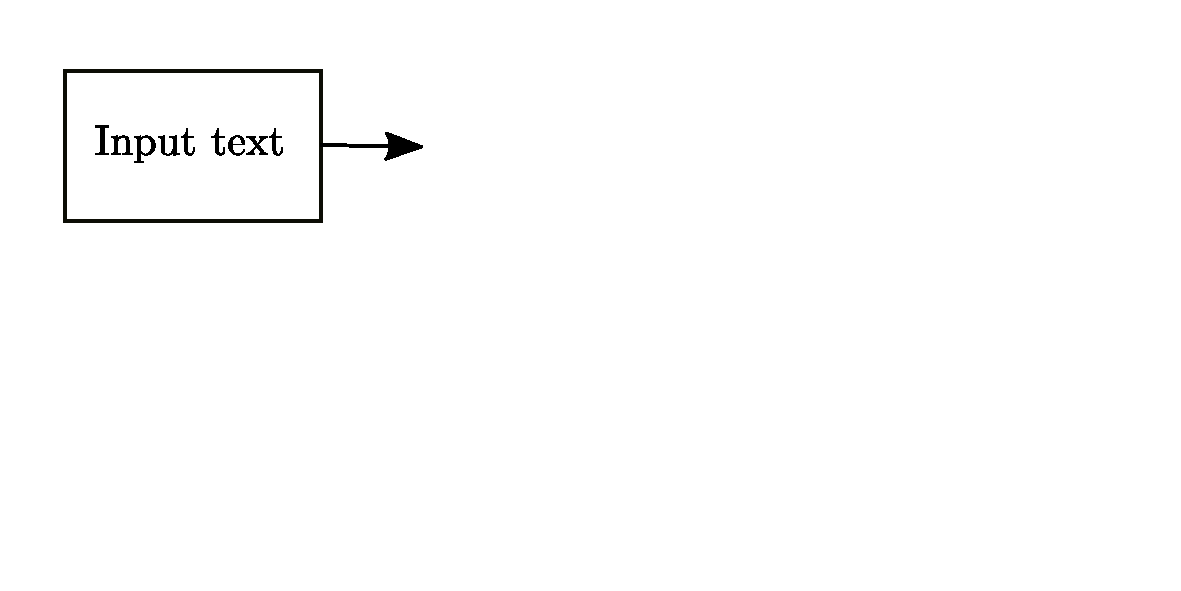
\includegraphics[scale=0.85]{NLP_pipeline}		
		%\captionsetup{justification=centering}
		\caption{The NLP pipeline}
		\label{NLP_pipeline_label}
	\end{figure}
	Let us just address briefly some possible points in the figure. Since sentence splitting produces sentences from an input text, the three arrows represent multiple sentences going into the tokenization block. As already said, it is important to know the sentence boundaries when computing the co-occurrence matrix. \\
	The tokenization block takes as an input the MWE block since it uses the MWE lexicon and other MWE specific features that we mentioned (e.g. abbreviations after the MWE) to correctly tokenize the input. \\
	And the last point to mention is the lemmatization block which takes in two inputs, the flow of tokens from the previous block and, to function properly, it also needs the PoS tags from the token removal block. \\
	This figure will be expanded once we talk about other steps required to build the whole model. 

	
	\newpage 
	\section{Word Embeddings}
	\subsection{How to Represent Words as Numbers?}
	The big challenge of any text processing on a computer is how to represent words as numbers? This is a fundamental question in NLP as computers inherently work with numbers and NLP works with words. In contrast to other areas of computer science like image processing and audio processing whose working medium (images and waveforms) can be and are represented with numbers, there is no apparent way on how to represent the working medium of NLP (words) as numbers. \\
	
	Of course, the naive approach would be to map each word in a language to a single number, but, for example, the word "banana" being number $134$ and the word "orange" being number $54$ doesn't tell us anything about those words or the relation between them. The thing is that a single number cannot represent the meaning of a word. The idea is to somehow represent the features of words. For example features of "orange" are that it is a fruit, round, orange colored, etc. In contrast a "banana" is also a fruit, it is curved and yellow. So in that sense, we could encode the features of words as number, and measure, for instance, how much is an object round or yellow and so on. The next natural step is to encode those feature of words as \textit{feature vectors} and this is the point where we come to word embeddings. \\
	
	\textbf{Word embeddings} are representation of words as dense real-valued vectors such that words which are closer in such a vector space tend to have a similar meaning \cite{word-embedding-survey}. Word embeddings have revolutionized the field of NLP by enabling computers to interpret and understand words. Each entry of the embedding represents a feature of the word. These vectors are in high-dimension spaces as there are tens and even hundreds of features that words have. The higher dimension the better representation of words we have, but there is the computational trade-off, as longer vectors required more resources to process and store. Let us look at an example $2$D subspace of a larger, high-dimensional space on how some words in such a space are behaving in terms of their embeddings in Figure \ref{subspace_label}.
	\begin{figure}[H]
		\centering
		\hspace*{-1.0cm}
		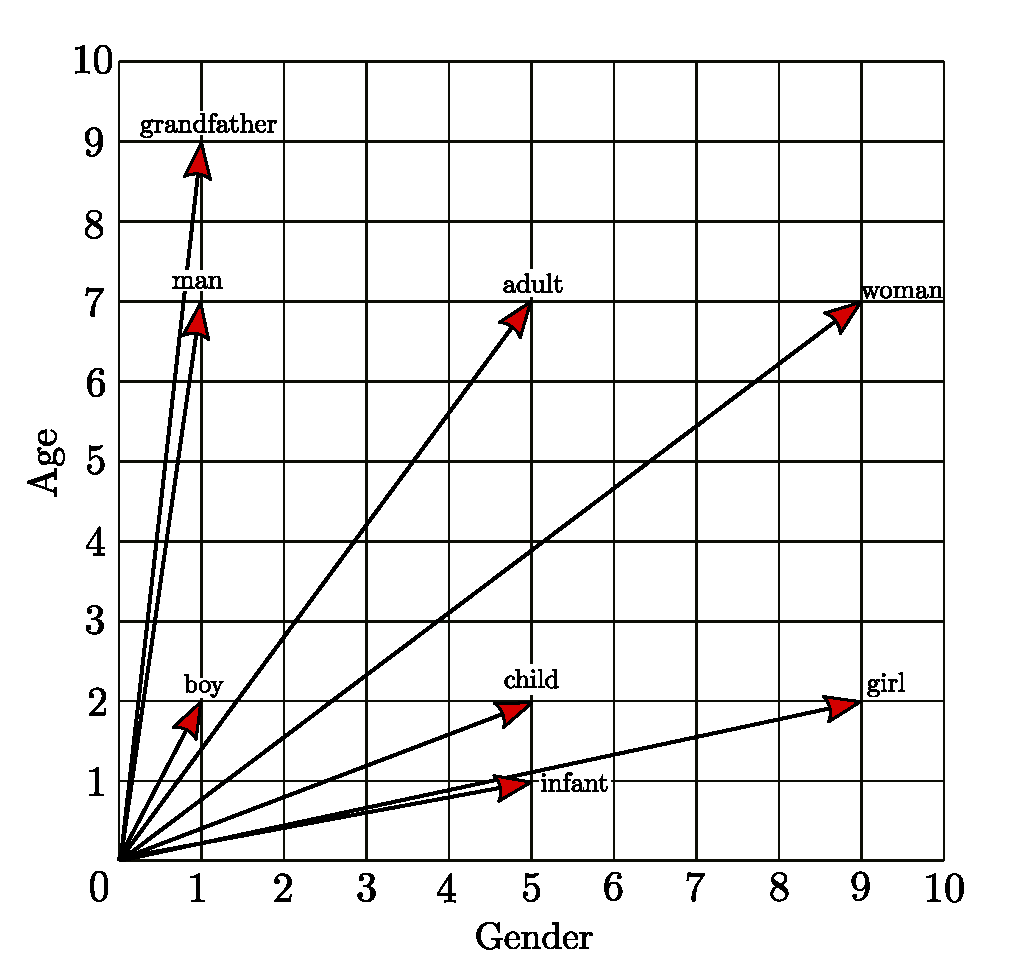
\includegraphics[scale=0.75]{subspace}		
		%\captionsetup{justification=centering}
		\caption{Word embeddings in the Gender-Age subspace}
		\label{subspace_label}
	\end{figure}
	
	The numbers on the Gender and Age axes are just for presentation purpose as word embeddings are usually real-valued which means they are also continuous. The reason for such a representation instead of an integer or one-hot representation is that continuous and dense vectors capture more accurate and subtle semantic relations between words. The other reason is that real-valued embeddings are more efficient for computation than other sparse representations. The vector elements are also usually in the range $[-1, 1]$ for normalization purposes when using them in neural networks. \\
	As for the example in Figure \ref{subspace_label} we can see that for the Gender axis the lower values are regarded as male (grandfather, man, boy), the higher values are regarded as female (woman, girl) and the values in between have no specific gender (adult, child, infant). As for the Age axis, we have the same idea, based on the age of person the words have higher or lower values. Here we see the power of embeddings, vector representations of words do really carry meaning with them. And if a new word would be mapped in this space, e.g. "lady" to the vector $(8, 6)$ based on how much the word is "old" or "young" and "male" or "female". We also see that words that are more similar are closer to each other in this space, and they form \textbf{clusters}. This is just a 2$D$ example of a space, but a space with, say $50$, dimensions have many more refined features and we can form more refined clusters (e.g. cluster of fruits which are yellow). In Figure \ref{cluster} we can see an example of different word clusters. One of the ways of obtaining these clusters is using the K-means clustering algorithm (in fact, it is the perfect example of using K-means). 
	\begin{figure}[H]
		\centering

		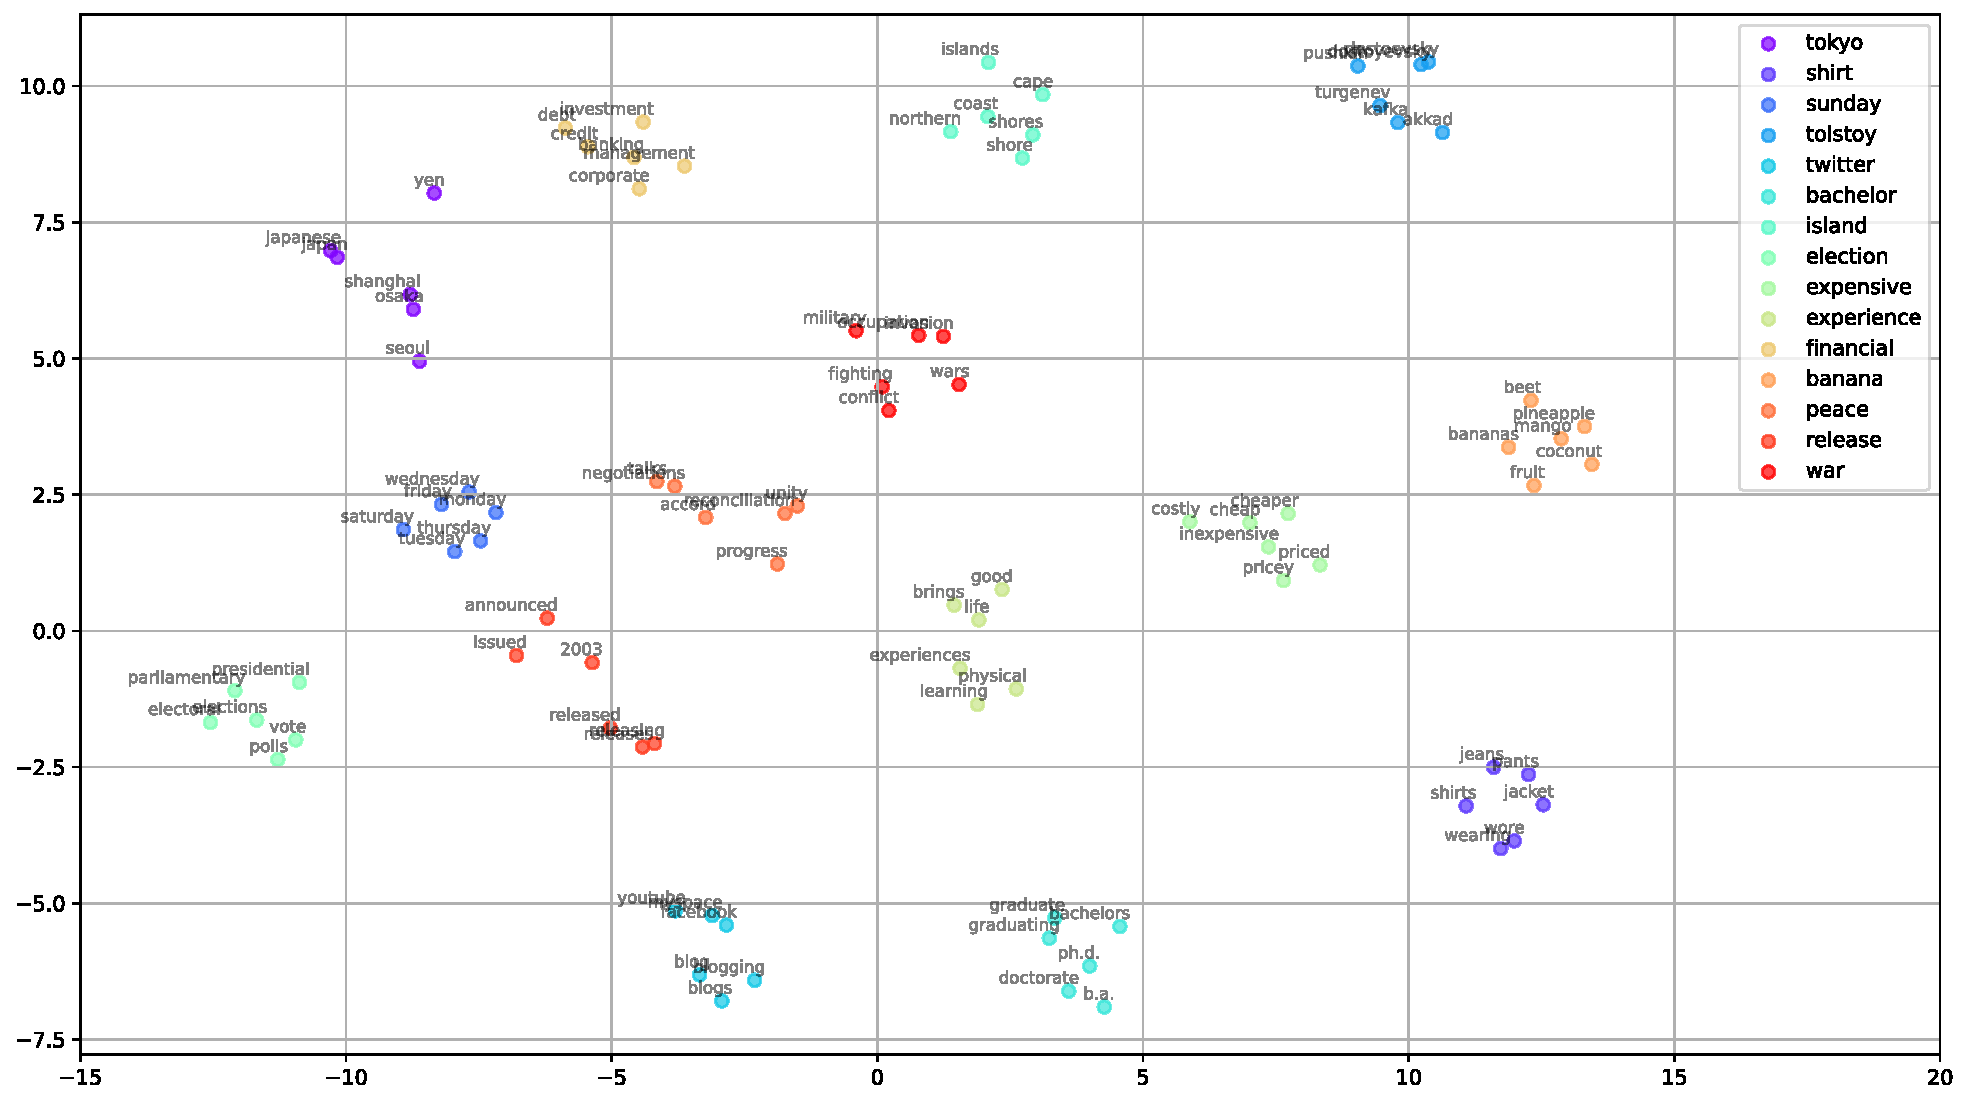
\includegraphics[scale=0.30]{clusters}		
		%\captionsetup{justification=centering}
		\caption{Clusters of words using word embeddings}
		\label{cluster}
	\end{figure}
% https://towardsdatascience.com/google-news-and-leo-tolstoy-visualizing-word2vec-word-embeddings-with-t-sne-11558d8bd4d
	
	The real power of these vectors is that we can perform standard vector operations on them, like the addition and the dot product. This enables us the numerically measure the similarity between word with the cosine similarity like:
	\begin{equation}\label{cosine_similarity}
		S_C(A, B) = \frac{\mathbf{A}\cdot \mathbf{B}}{\|\mathbf{A}\| \| \mathbf{B}\|}
	\end{equation}
	We can test this on the figure with the similarity between "grandfather" and "man" versus "grandfather" and "girl"
	$$ S_C(\text{grandfather}, \text{man}) = \frac{(1, 9) \cdot (1, 2)}{\|(1, 9)\| \|(1, 2)\|} = 0.94 $$ 
	$$ S_C(\text{grandfather}, \text{girl}) = \frac{(1, 9) \cdot (9, 2)}{\|(1, 9)\| \|(9, 2)\|} = 0.32 $$ 
	We observe the expected, that "grandfather" and "man" are more similar (both male and older) than "grandfather" and "girl" (different genders and ages). The other operation we mentioned was vector addition. Adding and subtracting word embeddings means that we basically add and subtract the features associated with words. Let us show that on an example (where WE means the word embedding of a word):
	$$ \text{WE}(\text{woman}) - \text{WE}(\text{man}) + \text{WE}(\text{boy}) = (9, 7) - (1,7) + (1, 2) = (9, 2) = \text{WE}(\text{girl})$$
	The intuition behind the addition and subtraction for this example is that we subtracted age from "woman" with the age of "man" (which gives $0$ age), and gender from "boy" with the gender of "man" (which gives $0$ gender) and added the age from "boy" and gender from "woman" which give us something that has an age of a boy and the gender of a woman. That something is a girl, which is exactly what we got. Doing this in higher dimensions we can get the closest cluster to the resulting vector and get all the words which are similar to the desired output.
	
	\subsection{How are Word Embeddings Calculated?}
	We have seen what word embeddings are, their functionalities and how to use them, but how do we actually get them, in an automated way? \\
	To core concept of obtaining word embeddings is that similar words occur in the same context. This means that words that are close together in a text also tend to be similar to each other. This is a strong assumption but it has been proven to be viable. The most successful models for calculating word embeddings are neural network based using the context assumption. The idea is to use a \textbf{skip-gram} model, which takes a target word and tries to predict the surrounding context words. We use a sliding window for the size of the context. Then the target word is used as the input to the neural network (actually the one hot encoded sliding window) and the context words are predicted as the output (which we know). The network is then trained to minimize the difference between the predicted and actual context words. The network weights are adjusted during the training to improve the accuracy of the predictions using the backpropagation algorithm. The resulting weights of the hidden layer are used as the word embeddings as they capture the semantic relationships between words. This skip-gram architecture is used in Google's \textbf{word2vec} word embeddings toolkit \cite{word2vec}. \\
	% https://medium.com/@corymaklin/word2vec-skip-gram-904775613b4c
	The other way of getting the embeddings is using global statistical information of the entire corpus constructing a co-occurrence matrix. That matrix represents the frequency of word pairs occurring together in a given context window. This is exactly the way we will get the pair-wise connections of nodes in the graph we will build. The obtained matrix is then factorized to the final embeddings (the process has some more details but we won't go into detail). This co-occurrence matrix architecture is used in the \textbf{GloVe} model \cite{glove}. 
	
	
	Word embedding calculation and storage (as dictionary)
	
	From words to phrases and beyond
	
	Homonymy with word embeddings
	
	How we are going to use them
	
	\newpage
	\section{Graph Construction}
	\subsection{Co-occurrence matrix}
	
	\newpage
	\section{Implementation of Keyword Extraction}
	
	\section{Testing, Results and Discussion}
	
	\subsection{Dataset}
	
	\section{Conclusion}
	
	\newpage
	\section{Literature}
	
	\begin{thebibliography}{8}
		\bibitem{word-embedding-survey}
		Almeida, Felipe, and Geraldo Xexéo. "\textit{Word embeddings: A survey}.", arXiv preprint arXiv:1901.09069 (2019). \\
		\texttt{URL: }\url{https://arxiv.org/pdf/1901.09069.pdf}
		
		\bibitem{transformers-survey}
		Lin, Tianyang, et al. "\textit{A survey of transformers}.", AI Open (2022).\\
		\texttt{URL: }\url{https://www.sciencedirect.com/science/article/pii/S2666651022000146}
		
		\bibitem{keyword-extraction-0}
		Zu, Xian, Fei Xie, and Xiaojian Liu. "\textit{Graph-based keyphrase extraction using word and document embeddings}.", 2020 IEEE International Conference on Knowledge Graph (ICKG). IEEE, 2020. \\
		\texttt{URL: }\url{https://ieeexplore.ieee.org/abstract/document/9194571}
		
		\bibitem{stanford_NLP}
		The Stanford NLP Group\\
		\texttt{URL: }\url{https://nlp.stanford.edu/}
		
		\bibitem{word2vec}
		Word2Vec project information\\
		\texttt{URL: }\url{https://code.google.com/archive/p/word2vec/}
		
		\bibitem{glove}
		GloVe: Global Vectors for Word Representation\\
		\texttt{URL: }\url{https://nlp.stanford.edu/projects/glove/}
		
		\bibitem{juricGrafovi}
		Jurić Ž. "\textit{Diskretna matematika za studente tehničkih nauka}". ETF Sarajevo, UNSA, 2017. 
		
	\end{thebibliography}

	\end{spacing}
	
\end{document}